% Options for packages loaded elsewhere
\PassOptionsToPackage{unicode}{hyperref}
\PassOptionsToPackage{hyphens}{url}
%
\documentclass[
  ,doc,floatsintext]{apa6}
\usepackage{amsmath,amssymb}
\usepackage{lmodern}
\usepackage{iftex}
\ifPDFTeX
  \usepackage[T1]{fontenc}
  \usepackage[utf8]{inputenc}
  \usepackage{textcomp} % provide euro and other symbols
\else % if luatex or xetex
  \usepackage{unicode-math}
  \defaultfontfeatures{Scale=MatchLowercase}
  \defaultfontfeatures[\rmfamily]{Ligatures=TeX,Scale=1}
\fi
% Use upquote if available, for straight quotes in verbatim environments
\IfFileExists{upquote.sty}{\usepackage{upquote}}{}
\IfFileExists{microtype.sty}{% use microtype if available
  \usepackage[]{microtype}
  \UseMicrotypeSet[protrusion]{basicmath} % disable protrusion for tt fonts
}{}
\makeatletter
\@ifundefined{KOMAClassName}{% if non-KOMA class
  \IfFileExists{parskip.sty}{%
    \usepackage{parskip}
  }{% else
    \setlength{\parindent}{0pt}
    \setlength{\parskip}{6pt plus 2pt minus 1pt}}
}{% if KOMA class
  \KOMAoptions{parskip=half}}
\makeatother
\usepackage{xcolor}
\IfFileExists{xurl.sty}{\usepackage{xurl}}{} % add URL line breaks if available
\IfFileExists{bookmark.sty}{\usepackage{bookmark}}{\usepackage{hyperref}}
\hypersetup{
  pdftitle={Friends or food: comparing social and food-based numerical cognition in captive pinyon jays},
  pdfauthor={London M. Wolff1},
  pdflang={en-EN},
  pdfkeywords={Numerical preference, Social cognition, Avian cognition},
  hidelinks,
  pdfcreator={LaTeX via pandoc}}
\urlstyle{same} % disable monospaced font for URLs
\usepackage{graphicx}
\makeatletter
\def\maxwidth{\ifdim\Gin@nat@width>\linewidth\linewidth\else\Gin@nat@width\fi}
\def\maxheight{\ifdim\Gin@nat@height>\textheight\textheight\else\Gin@nat@height\fi}
\makeatother
% Scale images if necessary, so that they will not overflow the page
% margins by default, and it is still possible to overwrite the defaults
% using explicit options in \includegraphics[width, height, ...]{}
\setkeys{Gin}{width=\maxwidth,height=\maxheight,keepaspectratio}
% Set default figure placement to htbp
\makeatletter
\def\fps@figure{htbp}
\makeatother
\setlength{\emergencystretch}{3em} % prevent overfull lines
\providecommand{\tightlist}{%
  \setlength{\itemsep}{0pt}\setlength{\parskip}{0pt}}
\setcounter{secnumdepth}{-\maxdimen} % remove section numbering
% Make \paragraph and \subparagraph free-standing
\ifx\paragraph\undefined\else
  \let\oldparagraph\paragraph
  \renewcommand{\paragraph}[1]{\oldparagraph{#1}\mbox{}}
\fi
\ifx\subparagraph\undefined\else
  \let\oldsubparagraph\subparagraph
  \renewcommand{\subparagraph}[1]{\oldsubparagraph{#1}\mbox{}}
\fi
\newlength{\cslhangindent}
\setlength{\cslhangindent}{1.5em}
\newlength{\csllabelwidth}
\setlength{\csllabelwidth}{3em}
\newlength{\cslentryspacingunit} % times entry-spacing
\setlength{\cslentryspacingunit}{\parskip}
\newenvironment{CSLReferences}[2] % #1 hanging-ident, #2 entry spacing
 {% don't indent paragraphs
  \setlength{\parindent}{0pt}
  % turn on hanging indent if param 1 is 1
  \ifodd #1
  \let\oldpar\par
  \def\par{\hangindent=\cslhangindent\oldpar}
  \fi
  % set entry spacing
  \setlength{\parskip}{#2\cslentryspacingunit}
 }%
 {}
\usepackage{calc}
\newcommand{\CSLBlock}[1]{#1\hfill\break}
\newcommand{\CSLLeftMargin}[1]{\parbox[t]{\csllabelwidth}{#1}}
\newcommand{\CSLRightInline}[1]{\parbox[t]{\linewidth - \csllabelwidth}{#1}\break}
\newcommand{\CSLIndent}[1]{\hspace{\cslhangindent}#1}
\ifLuaTeX
\usepackage[bidi=basic]{babel}
\else
\usepackage[bidi=default]{babel}
\fi
\babelprovide[main,import]{english}
% get rid of language-specific shorthands (see #6817):
\let\LanguageShortHands\languageshorthands
\def\languageshorthands#1{}
% Manuscript styling
\usepackage{upgreek}
\captionsetup{font=singlespacing,justification=justified}

% Table formatting
\usepackage{longtable}
\usepackage{lscape}
% \usepackage[counterclockwise]{rotating}   % Landscape page setup for large tables
\usepackage{multirow}		% Table styling
\usepackage{tabularx}		% Control Column width
\usepackage[flushleft]{threeparttable}	% Allows for three part tables with a specified notes section
\usepackage{threeparttablex}            % Lets threeparttable work with longtable

% Create new environments so endfloat can handle them
% \newenvironment{ltable}
%   {\begin{landscape}\centering\begin{threeparttable}}
%   {\end{threeparttable}\end{landscape}}
\newenvironment{lltable}{\begin{landscape}\centering\begin{ThreePartTable}}{\end{ThreePartTable}\end{landscape}}

% Enables adjusting longtable caption width to table width
% Solution found at http://golatex.de/longtable-mit-caption-so-breit-wie-die-tabelle-t15767.html
\makeatletter
\newcommand\LastLTentrywidth{1em}
\newlength\longtablewidth
\setlength{\longtablewidth}{1in}
\newcommand{\getlongtablewidth}{\begingroup \ifcsname LT@\roman{LT@tables}\endcsname \global\longtablewidth=0pt \renewcommand{\LT@entry}[2]{\global\advance\longtablewidth by ##2\relax\gdef\LastLTentrywidth{##2}}\@nameuse{LT@\roman{LT@tables}} \fi \endgroup}

% \setlength{\parindent}{0.5in}
% \setlength{\parskip}{0pt plus 0pt minus 0pt}

% Overwrite redefinition of paragraph and subparagraph by the default LaTeX template
% See https://github.com/crsh/papaja/issues/292
\makeatletter
\renewcommand{\paragraph}{\@startsection{paragraph}{4}{\parindent}%
  {0\baselineskip \@plus 0.2ex \@minus 0.2ex}%
  {-1em}%
  {\normalfont\normalsize\bfseries\itshape\typesectitle}}

\renewcommand{\subparagraph}[1]{\@startsection{subparagraph}{5}{1em}%
  {0\baselineskip \@plus 0.2ex \@minus 0.2ex}%
  {-\z@\relax}%
  {\normalfont\normalsize\itshape\hspace{\parindent}{#1}\textit{\addperi}}{\relax}}
\makeatother

% \usepackage{etoolbox}
\makeatletter
\patchcmd{\HyOrg@maketitle}
  {\section{\normalfont\normalsize\abstractname}}
  {\section*{\normalfont\normalsize\abstractname}}
  {}{\typeout{Failed to patch abstract.}}
\patchcmd{\HyOrg@maketitle}
  {\section{\protect\normalfont{\@title}}}
  {\section*{\protect\normalfont{\@title}}}
  {}{\typeout{Failed to patch title.}}
\makeatother

\usepackage{xpatch}
\makeatletter
\xapptocmd\appendix
  {\xapptocmd\section
    {\addcontentsline{toc}{section}{\appendixname\ifoneappendix\else~\theappendix\fi\\: #1}}
    {}{\InnerPatchFailed}%
  }
{}{\PatchFailed}
\keywords{Numerical preference, Social cognition, Avian cognition\newline\indent Word count: }
\usepackage{lineno}

\linenumbers
\usepackage{csquotes}
\usepackage{orcidlink}
\usepackage[justification=Centering,position=top]{subfig}
\ifLuaTeX
  \usepackage{selnolig}  % disable illegal ligatures
\fi

\title{Friends or food: comparing social and food-based numerical cognition in captive pinyon jays}
\author{London M. Wolff\textsuperscript{1}}
\date{}


\shorttitle{Numerical cognition in pinyon jays}

\authornote{

London M. Wolff, \orcidlink{0000-0001-8359-2619} \url{https://orcid.org/0000-0001-8359-2619}.

Correspondence concerning this article should be addressed to London M. Wolff, B83 East Stadium, University of Nebraska, Lincoln, Lincoln, NE, USA 68588. ORCID 0000-0003-2375-1360. E-mail: \href{mailto:lmwolff3@gmail.com}{\nolinkurl{lmwolff3@gmail.com}}

}

\affiliation{\vspace{0.5cm}\textsuperscript{1} Department of Psychology, Center for Brain, Biology \& Behavior, University of Nebraska, Lincoln, Lincoln, NE, USA}

\abstract{%
Animals must often discriminate different quantities of objects in their environment, from numbers of food items to conspecifics. Yet we know little about how this numerical cognition compares across different types of objects. Based on past research, we would expect individuals to use both numerical ratio and numerical difference to choose between two numerical options. This study investigates whether numerical ratio and difference predict numerical preference in pinyon jays (\emph{Gymnorhinus cyanocephalus}) for two types of stimuli, food items and conspecifics. Subjects (N=8 for food condition, N=10 for social condition) chose between two options using every paired combination of food item or group size number between 1 and 6. In both conditions, the pinyon jays showed an overall preference for the larger option over the smaller option. For the food condition, pinyon jays preferred numbers of items with higher numerical differences and lower numerical ratios. However, numerical difference did not influence preference independently of ratio. For the social condition, neither difference nor ratio predicted the subjects' choices. Thus, the pinyon jays showed different effects of numerical difference and ratio on preference across food items and conspecifics. One rationale for these results are pinyon jays use different strategies when deciding between numbers of food items and flock mates. While number is important for selecting food items, other factors such as flock mate identity may be more important for selecting social groups to join. Thus, in numerical preference situations, the type of objects offered drive the numerical strategies that animals use.
}



\begin{document}
\maketitle

\hypertarget{introduction}{%
\section{Introduction}\label{introduction}}

Many animal species have demonstrated the ability to quantify objects in their environment, including bees (Dacke \& Srinivasan, 2008), fish (Agrillo \& Dadda, 2007; Agrillo et al., 2008, 2011), amphibians (Uller et al., 2003), birds (Xia et al., 2001; Emmerton \& Renner, 2006, 2009), and mammals (Vonk \& Beran, 2012) but especially primates (Call, 2000; Beran, 2001; Nieder, 2018). As these animals are not closely related phylogenetically, some diverging hundreds of millions of years apart from each other (Nieder, 2018), quantification skills must have strong adaptive value. These adaptive benefits can be broken down into two main subgroups: benefits for survival and reproduction. Survival benefits include but are not limited to navigation, predator avoiding, territory defense, and cooperative hunting/foraging (Yang \& Chiao, 2016; Agrillo et al., 2017; Nieder, 2020). For example, wolves are more likely to capture a buffalo, if they cooperatively hunt in groups of 9-13 (MacNulty et al., 2014). Reproduction benefits of numerical competence include courtship, mating, and avoiding brood parasitism (Arak, 1983; White et al., 2009; Carazo et al., 2012). Having some form of numeric competence must be an important cognitive skill that incurs fitness benefits for survival and reproduction.

Two distinct cognitive systems, the object tracking system (OTS) and the approximate number system (ANS), are thought to describe how animals represent numbers (Hyde, 2011; Ditz \& Nieder, 2016). The object tracking system (OTS) is a visual mechanism that tracks up to four objects precisely while the approximate number system (ANS) is a mental system that supports the estimation of numerical quantity without relying on language or symbols (Nieder, 2020). The most important difference to highlight is that the OTS works on small (3 or 4) but precise numbers while the ANS works on approximate quantities of larger sizes (Feigenson et al., 2004; Nieder, 2020). Current literature demonstrates that animals will use the absolute number of items and therefore the OTS when assessing numerical stimuli in some cases(Cantlon \& Brannon, 2006; Emmerton \& Renner, 2006; Dacke \& Srinivasan, 2008). While animals use other cues such as surface area covered (Gómez-Laplaza \& Gerlai, 2013; Stancher et al., 2015), density (Bertamini et al., 2018; Gómez-Laplaza et al., 2019), or size of items (Stevens et al., 2007; Emmerton \& Renner, 2009) instead, of counting each object individually to estimate approximate quantities via the ANS.

Within the ANS, estimates are approximated through the use of numerical ratios and differences through the \emph{numerical magnitude effect} and the \emph{numerical distance effect} (Dehaene et al., 1998; Ditz \& Nieder, 2016). A numerical ratio is the mathematical quotient between two numbers: 2/4 has a ratio of 0.5. A numerical difference is the mathematical difference between two numbers: 4-2 has a difference of 2. The \emph{numerical magnitude effect} asserts that, at a given numerical difference, discrimination worsens with increasing magnitude, which is equivalent to a decreasing numerical ratio. Essentially, it becomes harder to discriminate as the numerical ratio approaches 1. The \emph{numerical distance effect} asserts that number discrimination improves with increasing numerical difference between two values. Essentially, it becomes easier to discriminate as the options become more dissimilar. Taken together, these two effects describe Weber's Law (Nieder, 2020). Quantity discriminations that follow Weber's law are a clear signature of the internal ANS and data showing difference and ratio effects illustrate the use of approximate amounts rather than precise numbers.

Past animal research investigating numerical cognition has found evidence that number is a relevant stimulus cue to which animals are sensitive across a number of contexts (Agrillo \& Beran, 2013; Agrillo \& Bisazza, 2014). Most of these numerical discrimination tasks use food or objects as stimuli (Call, 2000; Beran, 2001; Scarf et al., 2011; Rugani et al., 2013; Kelly, 2016). In previous studies, accuracy decreased as the ratio between the values approached 1, a direct confirmation of the \emph{numerical magnitude effect} (Cantlon \& Brannon, 2006; Hanus \& Call, 2007; Evans et al., 2009; Merten \& Nieder, 2009; Ditz \& Nieder, 2016). The second half of Weber's Law has been confirmed showing animals discriminate between a pair of numbers with more accuracy at larger numerical differences, \emph{numerical distance effect}, (Ditz \& Nieder, 2015, 2016; Tornick et al., 2015; Kelly, 2016). However, a subset of studies looking at fish use conspecifics (members of the same species) to assess numerical cognition (Buckingham et al., 2007; Agrillo et al., 2008; Gómez-Laplaza \& Gerlai, 2016). Many species prefer to be in larger groups, presumably because this dilutes their probability of being captured by predators (Krause \& Ruxton, 2002; Silk et al., 2014). Though some studies show an effect of both difference and ratio on social preference (Agrillo \& Dadda, 2007; Agrillo et al., 2008), others only show an effect of ratio (Buckingham et al., 2007; Gómez-Laplaza \& Gerlai, 2011). In all four of these conspecific item studies, subjects were better at discriminating ratios above one half than below. This is in accordance with the numerical magnitude effect, with only one of the four providing evidence that fish were capable of discriminating ratios below 1:2. Research shows ratio and difference effects in animals across contexts, yet no one has looked at context effects on numerical preference within a single test population of any one species.

Pinyon jays are well-suited for examining effects of context on numerical cognition because of their diet and social habits. Pinyon jays are a highly social species of North American corvid (Balda \& Kamil, 1998). They live in flocks ranging from 50 to 500 birds with fission-fusion dynamics in which members of a community form frequently changing subgroups (Balda \& Kamil, 1998; Wiggins, 2005; Lehmann et al., 2007). Fission-fusion group living reduces predation risk and improves foraging success (Lehmann et al., 2007; Dange et al., 2021). This is relevant to numerical cognition as birds in fission-fusion groups must often choose between breaking off into a smaller sub-group or rejoining the larger colony. One of the largest motivators of this decision-making process is foraging benefit (Silk et al., 2014). Pinyon jays forage for protein-rich pine nuts, which they cache to retrieve in the winter. 70 to 90\% of their winter diet is made up of cached seeds, even nestlings eat 10 to 32\% pine seeds (Balda \& Kamil, 1998). The need to retrieve cached food sources places strong selection pressure on numerical cognition, as they need to store as many pine seeds as possible to survive the winter. Pinyon jays rely on the quantity of food available for foraging decisions and the number of birds in a flock for social living decisions.

\hypertarget{present-study}{%
\subsection{Present Study}\label{present-study}}

The primary aim of the present study was to investigate how pinyon jays use numerical information, specifically numerical difference and ratio, to choose between different quantities of food items or conspecifics. To address this aim, we offered pinyon jays a series of choices between smaller and larger numbers of items: either high calorie treats (mealworms) or conspecifics.

To test our research question, we tested three hypotheses. Our first hypothesis (H1) posits that pinyon jays will, on average, prefer larger over smaller numbers of food items and conspecifics. An animal is more likely to survive, increasing their fitness outcome, if they consume more food. Similarity, an animal is more likely to survive by living in larger rather than smaller groups because they are decreasing the chance they will be killed by a predator. We hypothesize that pinyon jays would choose the larger flock as it increases your chances of finding a suitable mate and avoiding predators. Our second hypothesis (H2) posits that pinyon jays will show strong preferences for items with higher numerical differences and lower numerical ratios. As differences and ratios approach 1, the discrimination difficulty decreases. Discriminating between five and six mealworms is more difficult than discrimination between one and six. Our third hypothesis (H3) posits that both numerical difference and ratio will influence preference independently of each other. This distinction is important because difference and ratio are highly correlated with each other: as difference increases, ratio decreases. It is important to understand whether pinyon jays use difference, ratio, or both in a preference task to better understand how corvids make decisions across foraging and social domains.

\hypertarget{methods}{%
\section{Methods}\label{methods}}

\hypertarget{subjects}{%
\subsection{Subjects}\label{subjects}}

Our study population of 20 Pinyon Jays (\emph{Gymnorhinus cyanocephalus}) were wild born and locally housed. Researchers captured these birds in either Arizona or California (United States Fish and Wildlife permit MB694205) between 2006 and 2011. At capture, they were estimated to be between one and three years of age. The colony has an age range of 12 and 17 years with a mean of 14.45years . The University of Nebraska-Lincoln Institutional Animal Care and Use Committee approved this project (protocol number 1867 and 2059), and all procedures conformed to the ASAB/ABS Guidelines for the use of animals in research. All subjects have completed prior cognitive and behavioral experiments in their tenure with the lab.

Eight Pinyon Jays (one female) completed all rounds of the food experiment and 10 Pinyon Jays (four female) completed all rounds of the social experiment. The Pinyon Jays in the food item experiment were housed two to a double cage, while the jays in the social experiment were individually housed. A further 17 Pinyon Jays (six female) from the colony were used as stooge conspecifics in the social experiment. Two Pinyon Jays were dropped from the social experiment due to unrelated health concerns.

\hypertarget{food-experiment}{%
\subsection{Food Experiment}\label{food-experiment}}

\hypertarget{apparatus}{%
\subsubsection{Apparatus}\label{apparatus}}

The apparatus for the food experiment included a bird cage (72 x 48 x 48 cm) abutting a plastic stand with sliding trays that contained mealworms (Figure \ref{fig:foodapp}). Subjects started each trial perched on the large free standing perch, and then chose by landing on the smaller left or right perches. They then consumed the mealworms associated with their decision while the unchosen side was removed.



\begin{figure}

{\centering 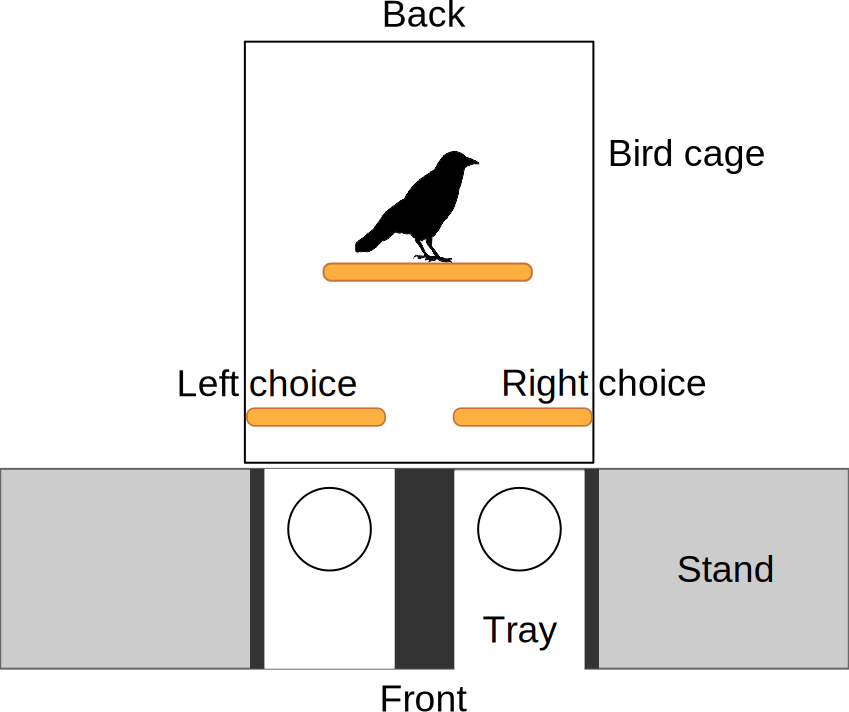
\includegraphics[width=1\linewidth]{../figures/food_apparatus} 

}

\caption{Food experiment apparatus (overhead view).}\label{fig:foodapp}
\end{figure}

\hypertarget{experimental-procedure}{%
\subsubsection{Experimental Procedure}\label{experimental-procedure}}

All experimental sessions ran between 11:00-13:00 CST to keep the birds' hunger levels constant throughout the experiment. The subjects were not food restricted and were fed three hours prior to the start of the experiment. The first trial of the session consisted of one round of mixed reward training. If they failed this check, the experimenter completed two more rounds of mixed reward training. If they failed two out of three of these trials this triggers de-bias training. If they succeed, they continued to the experimental trials. For these trials, the experimenter placed the appropriate number of mealworms in each of the dishes. The subject then started the trial on the back perch and hopped forward to one of the front perches to signal choice. The experimenter then removed the opposite dish and the subject had up to three minutes to consume their mealworms. Once the subject consumed all mealworms, we immediately started the next trial. If the subject did not make a choice and/or did not finish all mealworms within 3 minutes this triggered a stop on that days session.

Each bird experienced 10 repetitions for each of the 15 numerical pairs between 1 and 6 (e.g., 6 vs 5, 6 vs 4, 6 vs 3, etc.). The side of the larger option was pseudo randomized with no left or right runs longer than three in a row. Pairs were organized into 10 blocks. Each block was randomized within itself and had one instance of each factorial pair. Subjects order was randomized per session.

\hypertarget{social-experiment}{%
\subsection{Social Experiment}\label{social-experiment}}

\hypertarget{apparatus-1}{%
\subsubsection{Apparatus}\label{apparatus-1}}

The apparatus (Figure \ref{fig:socialapp}) took the form of a Y maze formed out of chicken wire, plastic sheets, and Plexiglas. The subject entered a large chamber at the base of the maze before choosing one of two arms of the Y maze. At the entrance to both arms, a guillotine style door was closed after the bird walked or flew past it, thus making a choice between the option on the left or right. At the end of each arm, was a large bird cage housing the stooge birds.



\begin{figure}

{\centering 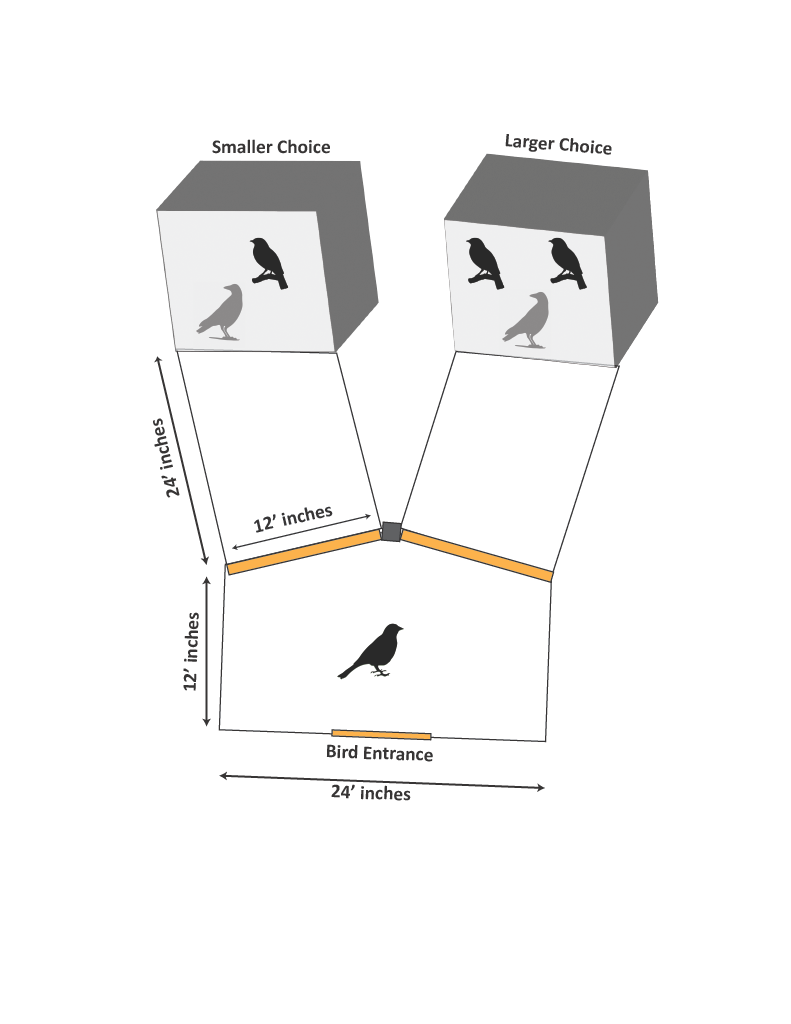
\includegraphics[width=1\linewidth]{../figures/social_apparatus} 

}

\caption{Social experiment apparatus (overhead view).}\label{fig:socialapp}
\end{figure}

\hypertarget{experimental-procedure-1}{%
\subsubsection{Experimental Procedure}\label{experimental-procedure-1}}

The subjects were not food restricted. The handler placed the subject inside the apparatus and showed them each option for six seconds before releasing the subject into the chamber. Once the subject crossed the threshold of one of the doors, the recorder closed \emph{both} doors gently but swiftly. After three minutes elapsed, the handler collected the subject and returned them to their home cage. These steps repeated until all birds had run through the experiment.

Each subject experienced 5 trials for each of the 21 numerical pairs between 0 and 6 (e.g., 6 vs 5, 6 vs 4, 6 vs 3, etc.). The side of the larger option was pseudo randomized with no left or right runs longer than 3 in a row. The pairs were organized into blocks with one instance of each pair per block and pairs randomized within each block. Subjects order was randomized per session.

\hypertarget{data-analysis}{%
\section{Data Analysis}\label{data-analysis}}

Data were analyzed and processed for the project using R (Version 4.2.1; R Core Team, 2021) and the R-packages \emph{BayesFactor} (Version 0.9.12.4.4; Morey \& Rouder, 2018), \emph{bayestestR} (Version 0.12.1; Makowski et al., 2019), \emph{BMA} (Version 3.18.17; Raftery et al., 2021), \emph{broom} (Version 1.0.0; Robinson et al., 2021), \emph{coda} (Version 0.19.4; Plummer et al., 2006), \emph{dplyr} (Version 1.0.9; Wickham et al., 2021), \emph{forcats} (Version 0.5.1; Wickham, 2021a), \emph{formattable} (Version 0.2.1; Ren \& Russell, 2021), \emph{ggplot2} (Version 3.3.6; Wickham, 2016), \emph{here} (Version 1.0.1; Müller, 2020), \emph{inline} (Version 0.3.19; Sklyar et al., 2021), \emph{knitr} (Version 1.39; Xie, 2015), \emph{leaps} (Version 3.1; Fortran code by Alan Miller, 2020), \emph{lme4} (Version 1.1.30; Bates et al., 2015), \emph{Matrix} (Version 1.4.1; Bates \& Maechler, 2021), \emph{papaja} (Version 0.1.1; Aust \& Barth, 2020), \emph{patchwork} (Version 1.1.1; Pedersen, 2020), \emph{performance} (Version 0.9.1; Lüdecke et al., 2021), \emph{purrr} (Version 0.3.4; Henry \& Wickham, 2020), \emph{readr} (Version 2.1.2; Wickham \& Hester, 2021), \emph{readxl} (Version 1.4.0; Wickham \& Bryan, 2019), \emph{robustbase} (Version 0.95.0; Todorov \& Filzmoser, 2009a), \emph{rrcov} (Version 1.7.0; Todorov \& Filzmoser, 2009b), \emph{stringr} (Version 1.4.0; Wickham, 2019), \emph{survival} (Version 3.3.1; Terry M. Therneau \& Patricia M. Grambsch, 2000), \emph{tibble} (Version 3.1.7; Müller \& Wickham, 2021), \emph{tidyr} (Version 1.2.0; Wickham, 2021b), \emph{tidyverse} (Version 1.3.1; Wickham et al., 2019), and \emph{tinylabels} (Version 0.2.3; Barth, 2022). Both the social and food stimuli data sets were analyzed using the same pre-registered analyses.

Throughout this paper, we will draw inferences based on Bayesian statistics (\emph{BF} values), as opposed to frequentist stats (\emph{p} values). While frequentist statistics are more prevalent in the current literature, we use Bayes statistics because they offer bidirectional information about both the alternative and the null hypotheses. That is, Bayes factors are the ratio of evidence for H\textsubscript{1} over evidence for H\textsubscript{0} (Wagenmakers, 2007; Wagenmakers et al., 2010). Therefore, a Bayes factor of 3 indicates three times more evidence for H\textsubscript{1} than H\textsubscript{0}, whereas a Bayes factor of 1/3 (the reciprocal of 3) indicates 3 times more evidence for H\textsubscript{0} than H\textsubscript{1}. We interpreted Bayes factors based on Wagenmakers et al. (2018), where a \emph{BF} \textgreater{} 3 is sufficient evidence for the alternative hypothesis, \emph{BF} \textless{} 1/3 is sufficient evidence for the null hypothesis, and 1/3 \textless{} \emph{BF} \textless{} 3 indicate neither hypothesis has evidence supporting it (suggesting the sample size is too small to draw conclusions).

Prior to analysis, we transformed the left and right choice variable from each trial into a binary operator, with 1 representing a choice for the larger option and 0 representing a choice for the smaller option. We also created variables with the numerical difference between each number pair by subtracting the larger number from the smaller (6-1 = 5), as well as creating the ratio by dividing the smaller by the larger number (1/6 = 0.16). Our hypotheses explore the relationship between our binary outcome variable, choice of the larger or smaller stimuli, and which possible mechanism, difference or ratio, subjects use to make choices when presented with either food or social items.

Our first hypothesis investigated whether pinyon jays prefer larger over smaller numbers of food items and conspecifics. To test this, we conducted a one sample t-tests of preference for larger numbers. Therefore, we calculated the mean \emph{percent preference for larger numbers} for each subject and used the t-test to compare the subject means to 50. We perform both frequentist and Bayesian t-tests, with inferences based on Bayes factors. Bayes factors for t-tests were calculated using the \texttt{ttestBF} function from the \emph{BayesFactor} R package (Morey et al., 2021) using default, noninformative priors.

Our second hypothesis investigated whether numerical difference and ratio predict preferences between smaller and larger options and the third hypothesis investigated whether difference and ratio predicted preferences \emph{independently}. To test these hypotheses, we used generalized linear mixed-effects modeling because the response variable was dichotomous and our subjects repeatedly made decision on the same number pairs. We used the trial-level choices for either the larger (coded as 1) or smaller (coded as 0) option available in the number pair as the response variable. To investigate our hypotheses, we used generalized logistic models to compare which combination of random (subject, pair, or both) and fixed (ratio, difference, or a combination of both) effects best describe each data set (food and social). We first found the best-fitting random effect structure, then added this random structure to all of the possible fixed effect structures, leaving us with the final best fitting model for each data set overall.

To explore random effect structure, we included models with no fixed effect and either (1) no random effects (intercept only), (2) subject as a random effect, (3) number pair as a random effect (to account for each bird repeatedly seeing each pair multiple times), and (4) both subject and number pair as random effects. For example, the model with both subject and pair as random effects ran using the \texttt{glmer()} function with the following structure: \texttt{r\ glmer(choice\ \textasciitilde{}\ (1\textbar{}subject)+\ (1\textbar{}pair),\ family\ =\ binomial)} (Figure \emph{A1} a). We then used Bayes factors to select the model with the best-fitting random effect structure. We added the chosen random effect structure to our fixed effects to find the best-fitting model for the data set overall. The five fixed effects models were: (1) no fixed effects (intercept only), (2) ratio as a fixed effect, (3) difference as a fixed effect, (4) both difference and ratio as a fixed effects but \emph{without} an interaction, and (5) both difference and ratio as fixed effects \emph{with} an interaction. The model with both difference and ratio as fixed effects with an interaction term ran using the \texttt{glm()} function and the following structure: \texttt{r\ glm(choice\ \textasciitilde{}\ difference\ *\ ratio,\ family\ =\ binomial)} (Figure \emph{A1} b). We calculated Bayes factors using the \texttt{test\_performance()} function from the \emph{performance} package (\emph{Performance}, 2021), which estimates Bayes factors from model BIC values using Wagenmakers' (Wagenmakers, 2007) equation. The best fitting model has the highest Bayes factor. The second hypothesis will be supported if difference and ratio are both included as main effects in the best fitting model. The third hypothesis will be supported if the interaction between difference and ratio is included in the best fitting model.

\hypertarget{results}{%
\section{Results}\label{results}}

\hypertarget{food-experiment-1}{%
\subsection{Food Experiment}\label{food-experiment-1}}

Our first hypothesis predicted that subjects would choose the larger number of mealworms over the smaller number of mealworms within any given pair across all sessions. On average, our subjects in the food study chose the larger option 60.75\% of the time with a standard deviation of 6.31. Results from a one sample t-test provided strong evidence that our hypothesis was supported (\(M = 60.75\), 95\% CI \([55.48, 66.02]\), \(t(7) = 4.82\), \(p = .002\), \(\mathrm{BF}_{\textrm{10}} = 24.28\)).

To investigate our other two hypotheses, we used model selection with mixed effect models. Hypothesis two predicts that (H2) pinyon jays prefer higher differences and lower ratios. If difference and ratio are both included as main effects in the best fitting model than hypothesis two will be supported. Hypothesis three predicts that (H3) difference and ratio are independent. If the interaction between difference and ratio is included in the best fitting model than this hypothesis three will be supported. We used a two-stage model selection approach that first selected the best random effects structure before investigating fixed effects. To determine the best random-effects structure, we compared models with all possible random effect combinations: subject, pair, and both subject and pair against the intercept only model. The model with the largest Bayes factor was assumed to have the best fit.

The best-fitting random effect structure for the food item data was the intercept only model, or no random effect structure, by rule of parsimony. The inclusion of only subject as a random effect (\(\mathrm{BF}_{\textrm{10}} = 0.15\)) was under 0.33, providing evidence that this random effect structure was not supported by the data. The inclusion of pair (\(\mathrm{BF}_{\textrm{10}} = 0.31\)), or both subject and pair (\(\mathrm{BF}_{\textrm{10}} = 0.06\)), also did not improve model fit. Therefore, we included no random effect structure in the second stage of comparisons looking at fixed effects. The five fixed effect model structures we compared included the (1) intercept only model against the model with (2) ratio as a fixed effect, (3) difference as a fixed effect, (4) both difference and ratio as a fixed effects but \emph{without} an interaction, and (5) both difference and ratio as fixed effects \emph{with} an interaction. The model with only the main effect of ratio (\(\mathrm{BF}_{\textrm{10}} = 1.87 \times 10^{3}\)) best fit the data out of the five models that we compared. The model with the second-best fit was the difference only model. To ensure that the ratio only model was the best fitting model we compared the ratio only and difference only models to find 4.08 times the evidence for the ratio only model as the difference only model. Thus, subjects in the food study used the ratio between the two numbers of mealworms to choose between options, with stronger preferences for larger options at smaller ratios (Figure \ref{fig:foodgraphs} a). Consequently, this only partially supports our second hypothesis, since difference was not included in the best fitting model (Figure \ref{fig:foodgraphs} b). Additionally, our third hypothesis was not supported, as the interaction term between difference and ratio was not included in the best fitting model (Figure \ref{fig:foodgraphs} c).



\begin{figure}

{\centering 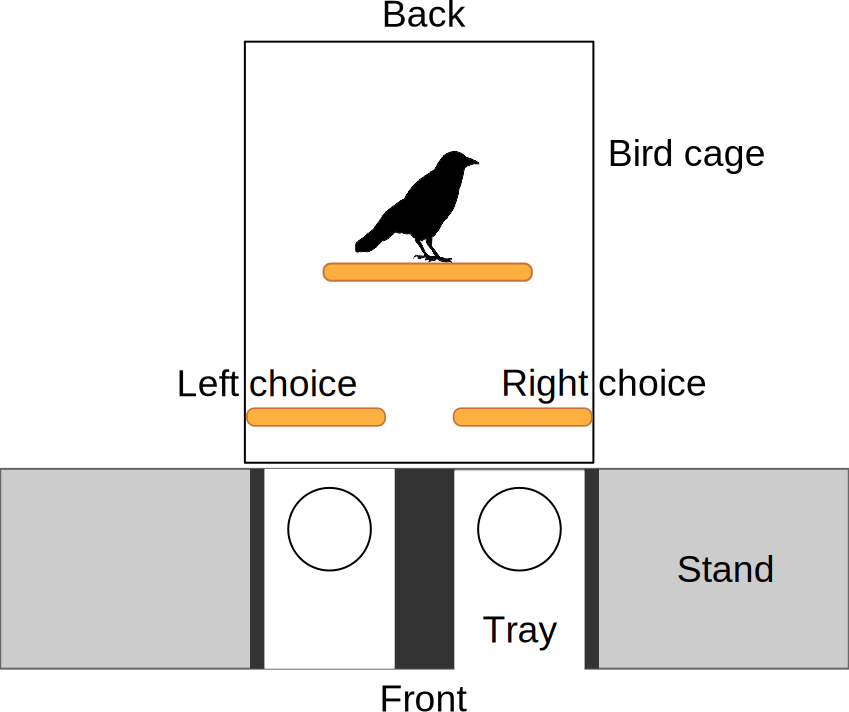
\includegraphics[width=1\linewidth]{../figures/food_apparatus} 

}

\caption{Food study difference, ratio, and interaction results (a) Mean preference for the larger option is shown on the y axis with the numerical difference options on the x axis. (b) Mean preference for the larger option is shown on the y axis with the numerical ratio options on the x axis. Dots represent mean values across all subjects and trials and error bars represent 95\% within-subject confidence intervals. Lines represent individual birds (N=8). (c) Mean preference for the larger option is shown on the y axis numerical ratio options on the x axis. The ratios were then grouped into the five numerical differences they represent. Dots represent mean values across all subjects and trials within a study.}\label{fig:foodgraphs}
\end{figure}

\hypertarget{social-experiment-1}{%
\subsection{Social Experiment}\label{social-experiment-1}}

Our first hypothesis predicted that subjects would choose the larger number of flock mates over the smaller number of flock mates within any given pair across all sessions. On average, our subjects in the social study choose the larger option 54.83\% of the time with a standard deviation of 4.67. Results from a one sample t-test provided moderate evidence that our hypothesis was supported (\(M = 54.83\), 95\% CI \([51.48, 58.17]\), \(t(9) = 3.27\), \(p = .010\), \(\mathrm{BF}_{\textrm{10}} = 6.33\)).

Results progressed similarly for the social study, we tested all possible random effects (subject, pair, and both) against the intercept only model to determine which, if any, of these random effects should be used in the full model.. Model testing revealed that the best-fitting random effect structure for the flock mate study no random effect structure. The inclusion of subject (\(\mathrm{BF}_{\textrm{10}} = 0.04\)), pair (\(\mathrm{BF}_{\textrm{10}} = 0.22\)), or both subject and pair (\(\mathrm{BF}_{\textrm{10}} = 0.01\)), did not improve the fit of the empty random effect model. All models had Bayes factors below 1/3, which provides evidence for the null hypothesis of the intercept only model. The intercept only model with a Bayes factor of 1 is the chosen random effect structure by rule of parsimony as it is the least complex model, therefore no random effect structure was added to our fixed effect models for the social study.

The same fixed effect structures were used in the social as the food study: an empty model, a model with only difference, only ratio, both but no interaction, and one model with both difference and ratio and an interaction. The intercept only model (\(\mathrm{BF}_{\textrm{10}} = 0.11\)) best fit the data by rule of parsimony. Similarly, to the random effect model structures, our fixed effect models also had Bayes factors less than 1/3. The model with the second best fit was the difference only model (\(\mathrm{BF}_{\textrm{10}} = 0.11\)), then the ratio only model (\(\mathrm{BF}_{\textrm{10}} = 0.32\)), both (\(\mathrm{BF}_{\textrm{10}} = 0.01\)), and the full model with an interaction (\(\mathrm{BF}_{\textrm{10}} = 0.00\)). Because ratio and difference failed to predict choices, neither of our hypothesis were supported by the data (Figure \ref{fig:socialgraphs}). Subjects did not use difference or ratio to make numerical decisions about conspecifics.



\begin{figure}

{\centering 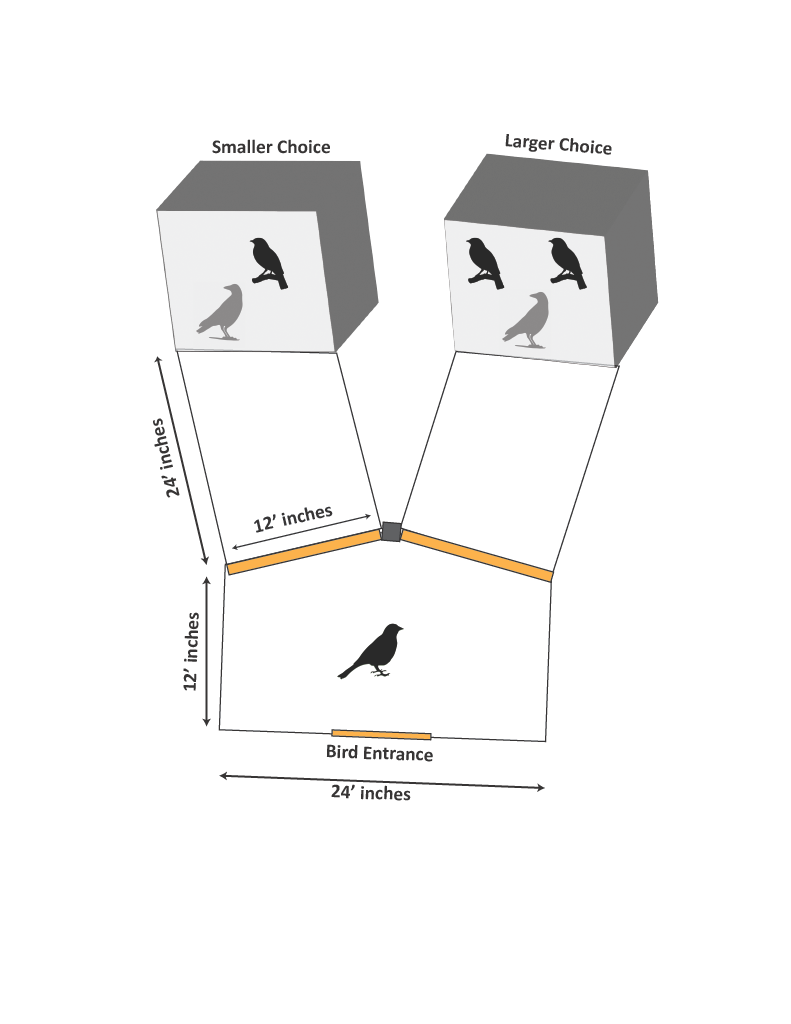
\includegraphics[width=1\linewidth]{../figures/social_apparatus} 

}

\caption{Social study difference, ratio, and interaction results (a) Mean preference for the larger option is shown on the y axis with the numerical difference options on the x axis. (b) Mean preference for the larger option is shown on the y axis with the numerical ratio options on the x axis. Dots represent mean values across all subjects and trials and error bars represent 95\% within-subject confidence intervals. Lines represent individual birds (N=10). (c) Mean preference for the larger option is shown on the y axis numerical ratio options on the x axis. The ratios were then grouped into the five numerical differences they represent. Dots represent mean values across all subjects and trials within a study.}\label{fig:socialgraphs}
\end{figure}

\hypertarget{discussion}{%
\section{Discussion}\label{discussion}}

We examined pinyon jays' numerical cognitive abilities in a food and social preference task. In both studies birds chose the larger of the two options on average across trials confirming our first hypothesis. In the food study, smaller numerical ratios but not larger numerical differences predicted the birds' choices partially confirming our second hypothesis. In the social experiment, neither ratio nor difference predicted choice showing that our second hypothesis was unsupported. In both the food and social experiments, difference and ratio did not independently predict choice indicating that our third hypothesis was also unsupported across studies. In neither context do pinyon jays use both ratio and difference together to choose between flock mates or food items

Results from the food study align with previous corvid research that birds prefer larger over smaller quantities and smaller ratios (Tornick et al., 2015; Ditz \& Nieder, 2016; Kelly, 2016). This ratio effect supports our theory that preference for the larger option decreases as the ratio between the values approaches 1, confirming that birds acted in accordance with the \emph{numerical magnitude effect}. Therefore, we have evidence supporting subjects using the approximate number system as a mechanism for quantity discrimination. Pinyon jays use amount of food, rather than precise number. However, the \emph{numerical distance effect} was not present in our data as number preference did not increase as difference increased between two values. See limitations for further comment on this outcome.

Our lack of significant findings in the social study suggests that pinyon jays do not have just one mechanism they use across contexts. While ratio was shown to be an important mechanism to pinyon jays when foraging, neither difference nor ratio were the mechanism of choice when choosing between flock mates. This outcome is surprising as previous numeric discrimination tasks with conspecifics found effects of difference and ratio (Agrillo \& Dadda, 2007; Agrillo et al., 2008). However, these experiments were completed in fish, not corvids. Corvids have a more complex system of sociality (Balda \& Kamil, 1998). Possibly, individual identity of birds overrides the implicit need to go to the smaller ratio and larger difference. Work in geese indicate that movement patterns of individuals may be shaped by the personality types present in the group (Kurvers et al., 2009). Furthermore, when testing Mexican Jay's on food item discrimination in the presence of flock mates, (Kelly, 2016) found no significant effect of ratio or difference as the birds were more likely to follow the previous bird, than pick the food item of a larger quantity. Possibly, this is because observing conspecifics provides important information, such as the safety of a food patch or resource availability (Krause et al., 2010; Handegard et al., 2012). Taken together, this suggests that birds do no view conspecifics in the same numeric terms as other objects and further investigation is needed to understand what internal systems animals are using to make numerical choices about conspecifics.

The differences in numerical preference between food and social contexts may be due to different selective pressures. Both flock size and foraging techniques have consequences for evolutionary fitness, but they tackle different adaptive problems. Food consumption acts primarily via natural selection by enhancing survival. Flock size, however, is integral to both natural and sexual selection: natural selection in the form of predator evasion, and sexual selection in the form of mate preference/reproduction. Joining a larger flock size allows an animal to dilute their chances of being eaten by predators (i.e., the dilution effect). Predator evasion acts on natural selection, allowing the animal to live long enough to reproduce, propagating its genes into the next generation. This selection pressure could account for our lack of difference and ratio findings in the flock mate experiment. Instead of using numerical difference and ratio to optimize predator evasion, birds are more likely focused on other biological imperatives like finding a suitable mate. Based on our current data, it seems that when choosing between two flocks, birds are making decision not based on the number of animals on each side but rather the identity of the animals. For example, a female bird should go to the flock option with suitable males, aligning with sexual selection mechanisms, over optimizing predator evasion. It is these evolutionary differences that could account for the variation we see in numerical cognitive strategies.

It is important to highlight that these results correspond to a numerical \emph{preference} task, not a discrimination task. If a subject discriminates between two objects, that means they recognize them as different. Preference denotes a liking of one option over the other. Meaning, the lack of a preference between two numbers of objects does not mean that the subject cannot discriminate the two objects. They just might not care about the difference. If a bird chooses indiscriminately between 5 or 6 mealworms it may not mean that they cannot discriminate between 5 and 6, but rather they are equally preferred. A clear preference implies discrimination, but lack of a preference does not imply an absence of discrimination.

To be clear, we are not making any claims about the method by which the birds make these preference-based numerical choices. That is, our study does not allow us to distinguish between the birds choosing larger \emph{numbers} of food items or conspecifics and larger \emph{amounts} of them. Previous studies have shown that instead of the absolute number, animals often make decisions based on the surface area or item size available (Gómez-Laplaza \& Gerlai, 2013; Gómez-Laplaza et al., 2019). For example, in our study, subjects could have chosen an option because they have a preference for 10\% of a tray covered by mealworms over another with only 7\% of the tray covered as opposed to preferring six over four mealworms. It is possible surface area, density, or quantity were all possible methods used by the subjects to make the numerical decisions discussed in the paper. In the food item study, total quantity is a reasonable criteria because the birds ultimate goal is to obtain as much food as possible to stay alive (e.g.~two large mealworms are better than 3 small mealworms). Therefore, total calories or overall food intake, rather than absolute number, is a better evolutionary strategy. Future work is needed to tease apart which methods birds use when presented with food or conspecifics.

\hypertarget{limitations}{%
\subsection{Limitations}\label{limitations}}

Though numerical ratio predicted choice in the food study, it did not in the social study, and difference did not predict choice in either study. This result was unlike previous corvid research, which found both difference and ratio effects in food studies (Tornick et al., 2015; Ditz \& Nieder, 2016; Kelly, 2016). This could be due to the limited range within our pair options. The smallest difference option we offered subjects was one (2-1=1) and the largest was five (6-1=5).Previous studies difference options ranged from 8 as the largest option offered to 30 (Tornick et al., 2015; Ditz \& Nieder, 2016). Considering that pinyon jay flock sizes range from 50 to 500 (Wiggins, 2005), the limited range of difference options may not have provided enough opportunities to demonstrate effects of difference.

\hypertarget{conclusion}{%
\subsection{Conclusion}\label{conclusion}}

The present research investigated how pinyon jays assess numbers of food items and conspecifics in a preference task. We showed that overall, pinyon jays chose the larger option over the smaller in both contexts. In a food context, pinyon jays use numerical ratio but \emph{not} numerical difference to make decisions. In a social context, subjects did not use difference or ratio to make decisions. Taken together, our findings suggest that while number or amount is important for selecting food items, other factors such as flock mate identity may be more important for selecting social groups to join. Thus, in numerical preference situations, the type of objects offered drive the numerical strategies that animals use.

\hypertarget{acknowledgments}{%
\subsection{Acknowledgments}\label{acknowledgments}}

This research was funded by National Science Foundation grants (NSF-1062045,
NSF-1658837). We would like to thank Kylie Hughes and Katie Carey our amazing lab managers for collecting data and helping the lab run smoothly and our RA's: Toria Biancalana, Hailey Wilson, Bailey Wilson, Isaac Martinez, and Rachel Bruner for collecting data.

\hypertarget{ethics-approval}{%
\subsection{Ethics approval}\label{ethics-approval}}

All procedures were conducted in an ethical and responsible manner, in full compliance with all relevant codes of experimentation and legislation and were approved by the UNL Internal Review Board (protocol \# 17922) and Institutional Animal Care and Use Committee (protocol \# 1621).

\newpage

\hypertarget{references}{%
\section{References}\label{references}}

\hypertarget{refs}{}
\begin{CSLReferences}{1}{0}
\leavevmode\vadjust pre{\hypertarget{ref-Agrillo.Beran.2013}{}}%
Agrillo, C., \& Beran, M. J. (2013). Number without language: Comparative psychology and the evolution of numerical cognition. \emph{Frontiers in Psychology}. \url{https://www.academia.edu/6879466/Number_without_language_comparative_psychology_and_the_evolution_of_numerical_cognition}

\leavevmode\vadjust pre{\hypertarget{ref-Agrillo.Bisazza.2014}{}}%
Agrillo, C., \& Bisazza, A. (2014). Spontaneous versus trained numerical abilities. {A} comparison between the two main tools to study numerical competence in non-human animals. \emph{Journal of Neuroscience Methods}, \emph{234}, 82--91. \url{https://doi.org/10.1016/j.jneumeth.2014.04.027}

\leavevmode\vadjust pre{\hypertarget{ref-Agrillo.Dadda.2007}{}}%
Agrillo, C., \& Dadda, M. (2007). Discrimination of the larger shoal in the poeciliid fish {Girardinus} falcatus. \emph{Ethology Ecology \& Evolution}, \emph{19}(2), 145--157. \url{https://doi.org/10.1080/08927014.2007.9522574}

\leavevmode\vadjust pre{\hypertarget{ref-Agrillo.etal.2008}{}}%
Agrillo, C., Dadda, M., Serena, G., \& Bisazza, A. (2008). Do fish count? {Spontaneous} discrimination of quantity in female mosquitofish. \emph{Animal Cognition}, \emph{11}(3), 495--503. \url{https://doi.org/10.1007/s10071-008-0140-9}

\leavevmode\vadjust pre{\hypertarget{ref-Agrillo.etal.2017}{}}%
Agrillo, C., Miletto Petrazzini, M. E., \& Bisazza, A. (2017). Numerical abilities in fish: {A} methodological review. \emph{Behavioural Processes}, \emph{141}(Pt 2), 161--171. \url{https://doi.org/10.1016/j.beproc.2017.02.001}

\leavevmode\vadjust pre{\hypertarget{ref-Agrillo.etal.2011}{}}%
Agrillo, C., Piffer, L., \& Bisazza, A. (2011). Number versus continuous quantity in numerosity judgments by fish. \emph{Cognition}, \emph{119}(2), 281--287. \url{https://doi.org/10.1016/j.cognition.2010.10.022}

\leavevmode\vadjust pre{\hypertarget{ref-Arak.1983}{}}%
Arak, A. (1983). Vocal interactions, call matching and territoriality in a {Sri} {Lankan} treefrog, {Philautus} leucorhinus ({Rhacophoridae}). \emph{Animal Behaviour}, \emph{31}(1), 292--302. \url{https://doi.org/10.1016/S0003-3472(83)80199-7}

\leavevmode\vadjust pre{\hypertarget{ref-R-papaja}{}}%
Aust, F., \& Barth, M. (2020). \emph{{papaja}: {Create} {APA} manuscripts with {R Markdown}}. \url{https://github.com/crsh/papaja}

\leavevmode\vadjust pre{\hypertarget{ref-Balda.Kamil.1998}{}}%
Balda, R. P., \& Kamil, A. (1998). \emph{The {Ecology} and {Evolution} of {Spatial} {Memory} in {Corvids} of the {Southwestern} {USA}: {The} {Perplexing} {Pinyon} {Jay}}. 37.

\leavevmode\vadjust pre{\hypertarget{ref-R-tinylabels}{}}%
Barth, M. (2022). \emph{{tinylabels}: Lightweight variable labels}. \url{https://cran.r-project.org/package=tinylabels}

\leavevmode\vadjust pre{\hypertarget{ref-R-lme4}{}}%
Bates, D., Mächler, M., Bolker, B., \& Walker, S. (2015). Fitting linear mixed-effects models using {lme4}. \emph{Journal of Statistical Software}, \emph{67}(1), 1--48. \url{https://doi.org/10.18637/jss.v067.i01}

\leavevmode\vadjust pre{\hypertarget{ref-R-Matrix}{}}%
Bates, D., \& Maechler, M. (2021). \emph{Matrix: Sparse and dense matrix classes and methods}. \url{https://CRAN.R-project.org/package=Matrix}

\leavevmode\vadjust pre{\hypertarget{ref-Beran.2001}{}}%
Beran, M. (2001). Summation and numerousness judgments of sequentially presented sets of items by chimpanzees ({Pan} troglodytes). \emph{Journal of Comparative Psychology (Washington, D.C. : 1983)}, \emph{115}, 181--191. \url{https://doi.org/10.1037//0735-7036.115.2.181}

\leavevmode\vadjust pre{\hypertarget{ref-Bertamini.etal.2018}{}}%
Bertamini, M., Guest, M., Vallortigara, G., Rugani, R., \& Regolin, L. (2018). The effect of clustering on perceived quantity in humans ({Homo} sapiens) and in chicks ({Gallus} gallus). \emph{Journal of Comparative Psychology (Washington, D.C.: 1983)}, \emph{132}(3), 280--293. \url{https://doi.org/10.1037/com0000114}

\leavevmode\vadjust pre{\hypertarget{ref-Buckingham.etal.2007}{}}%
Buckingham, J. N., Wong, B. B. M., \& Rosenthal, G. G. (2007). Shoaling decisions in female swordtails: {How} do fish gauge group size? \emph{Behaviour}, \emph{144}(11), 1333--1346. \url{https://doi.org/10.1163/156853907782418196}

\leavevmode\vadjust pre{\hypertarget{ref-Call.2000}{}}%
Call, J. (2000). Estimating and operating on discrete quantities in {Orangutans} ({Pongo} pygmaeus). \emph{Journal of Comparative Psychology}, \emph{114}(2), 136--147. \url{https://doi.org/10.1037/0735-7036.114.2.136}

\leavevmode\vadjust pre{\hypertarget{ref-Cantlon.Brannon.2006}{}}%
Cantlon, J. F., \& Brannon, E. M. (2006). Shared {System} for {Ordering} {Small} and {Large} {Numbers} in {Monkeys} and {Humans}. \emph{Psychological Science}, \emph{17}(5), 401--406. \url{https://doi.org/10.1111/j.1467-9280.2006.01719.x}

\leavevmode\vadjust pre{\hypertarget{ref-Carazo.etal.2012}{}}%
Carazo, P., Fernández-Perea, R., \& Font, E. (2012). Quantity {Estimation} {Based} on {Numerical} {Cues} in the {Mealworm} {Beetle} ({Tenebrio} molitor). \emph{Frontiers in Psychology}, \emph{3}, 502. \url{https://doi.org/10.3389/fpsyg.2012.00502}

\leavevmode\vadjust pre{\hypertarget{ref-Dacke.Srinivasan.2008}{}}%
Dacke, M., \& Srinivasan, M. V. (2008). Evidence for counting in insects. \emph{Animal Cognition}, \emph{11}(4), 683--689. \url{https://doi.org/10.1007/s10071-008-0159-y}

\leavevmode\vadjust pre{\hypertarget{ref-Dange.etal.2021}{}}%
Dange, P., Mhaisalkar, P., \& Paranjpe, D. (2021). To group or not to group: Group size dynamics and intestinal parasites in {Indian} peafowl populations. \emph{Acta Ethologica}, \emph{24}(2), 107--117. \url{https://doi.org/10.1007/s10211-021-00366-x}

\leavevmode\vadjust pre{\hypertarget{ref-Dehaene.etal.1998}{}}%
Dehaene, S., Dehaene-Lambertz, G., \& Cohen, L. (1998). Abstract representations of numbers in the animal and human brain. \emph{Trends in Neurosciences}, \emph{21}(8), 355--361. \url{https://doi.org/10.1016/S0166-2236(98)01263-6}

\leavevmode\vadjust pre{\hypertarget{ref-Ditz.Nieder.2016}{}}%
Ditz, H. M., \& Nieder, A. (2016). Numerosity representations in crows obey the {Weber}--{Fechner} law. \emph{Proceedings of the Royal Society B: Biological Sciences}, \emph{283}(1827), 20160083. \url{https://doi.org/10.1098/rspb.2016.0083}

\leavevmode\vadjust pre{\hypertarget{ref-Ditz.Nieder.2015}{}}%
Ditz, H. M., \& Nieder, A. (2015). Neurons selective to the number of visual items in the corvid songbird endbrain. \emph{Proceedings of the National Academy of Sciences}, \emph{112}(25), 7827--7832. \url{https://doi.org/10.1073/pnas.1504245112}

\leavevmode\vadjust pre{\hypertarget{ref-Emmerton.Renner.2006}{}}%
Emmerton, J., \& Renner, J. C. (2006). Scalar effects in the visual discrimination of numerosity by pigeons. \emph{Learning \& Behavior}, \emph{34}(2), 176--192. \url{https://doi.org/10.3758/BF03193193}

\leavevmode\vadjust pre{\hypertarget{ref-Emmerton.Renner.2009}{}}%
Emmerton, J., \& Renner, J. C. (2009). Local rather than global processing of visual arrays in numerosity discrimination by pigeons ({Columba} livia). \emph{Animal Cognition}, \emph{12}(3), 511--526. \url{https://doi.org/10.1007/s10071-009-0212-5}

\leavevmode\vadjust pre{\hypertarget{ref-Evans.etal.2009}{}}%
Evans, T. A., Beran, M. J., Harris, E. H., \& Rice, D. F. (2009). Quantity judgments of sequentially presented food items by capuchin monkeys ({Cebus} apella). \emph{Animal Cognition}, \emph{12}(1), 97--105. \url{https://doi.org/10.1007/s10071-008-0174-z}

\leavevmode\vadjust pre{\hypertarget{ref-Feigenson.etal.2004}{}}%
Feigenson, L., Dehaene, S., \& Spelke, E. (2004). Core systems of number. \emph{Trends in Cognitive Sciences}, \emph{8}(7), 307--314. \url{https://doi.org/10.1016/j.tics.2004.05.002}

\leavevmode\vadjust pre{\hypertarget{ref-R-leaps}{}}%
Fortran code by Alan Miller, T. L. based on. (2020). \emph{Leaps: Regression subset selection}. \url{https://CRAN.R-project.org/package=leaps}

\leavevmode\vadjust pre{\hypertarget{ref-Gomez-Laplaza.Gerlai.2011}{}}%
Gómez-Laplaza, L. M., \& Gerlai, R. (2011). Can angelfish ({Pterophyllum} scalare) count? {Discrimination} between different shoal sizes follows {Weber}'s law. \emph{Animal Cognition}, \emph{14}(1), 1--9. \url{https://doi.org/10.1007/s10071-010-0337-6}

\leavevmode\vadjust pre{\hypertarget{ref-Gomez-Laplaza.Gerlai.2013}{}}%
Gómez-Laplaza, L. M., \& Gerlai, R. (2013). The role of body surface area in quantity discrimination in angelfish ({Pterophyllum} scalare). \emph{PloS One}, \emph{8}(12), e83880. \url{https://doi.org/10.1371/journal.pone.0083880}

\leavevmode\vadjust pre{\hypertarget{ref-Gomez-Laplaza.Gerlai.2016}{}}%
Gómez-Laplaza, L. M., \& Gerlai, R. (2016). Discrimination of large quantities: {Weber}'s law and short-term memory in angelfish, {Pterophyllum} scalare. \emph{Animal Behaviour}, \emph{112}, 29--37. \url{https://doi.org/10.1016/j.anbehav.2015.10.022}

\leavevmode\vadjust pre{\hypertarget{ref-Gomez-Laplaza.etal.2019}{}}%
Gómez-Laplaza, L. M., Romero, L., \& Gerlai, R. (2019). The role of item size on choosing contrasted food quantities in angelfish ({Pterophyllum} scalare). \emph{Scientific Reports}, \emph{9}(1), 15305. \url{https://doi.org/10.1038/s41598-019-51753-1}

\leavevmode\vadjust pre{\hypertarget{ref-Handegard.etal.2012}{}}%
Handegard, N. O., Boswell, K. M., Ioannou, C. C., Leblanc, S. P., Tjøstheim, D. B., \& Couzin, I. D. (2012). The {Dynamics} of {Coordinated} {Group} {Hunting} and {Collective} {Information} {Transfer} among {Schooling} {Prey}. \emph{Current Biology}, \emph{22}(13), 1213--1217. \url{https://doi.org/10.1016/j.cub.2012.04.050}

\leavevmode\vadjust pre{\hypertarget{ref-Hanus.Call.2007}{}}%
Hanus, D., \& Call, J. (2007). Discrete quantity judgments in the great apes ({Pan} paniscus, {Pan} troglodytes, {Gorilla} gorilla, {Pongo} pygmaeus): {The} effect of presenting whole sets versus item-by-item. \emph{Journal of Comparative Psychology}, \emph{121}(3), 241--249. \url{https://doi.org/10.1037/0735-7036.121.3.241}

\leavevmode\vadjust pre{\hypertarget{ref-R-purrr}{}}%
Henry, L., \& Wickham, H. (2020). \emph{Purrr: Functional programming tools}. \url{https://CRAN.R-project.org/package=purrr}

\leavevmode\vadjust pre{\hypertarget{ref-Hyde.2011}{}}%
Hyde, D. C. (2011). Two {Systems} of {Non}-{Symbolic} {Numerical} {Cognition}. \emph{Frontiers in Human Neuroscience}, \emph{5}, 150. \url{https://doi.org/10.3389/fnhum.2011.00150}

\leavevmode\vadjust pre{\hypertarget{ref-Kelly.2016}{}}%
Kelly, E. M. (2016). Counting on your friends: {The} role of social environment on quantity discrimination. \emph{Behavioural Processes}, \emph{128}, 9--16. \url{https://doi.org/10.1016/j.beproc.2016.03.019}

\leavevmode\vadjust pre{\hypertarget{ref-Krause.Ruxton.2002}{}}%
Krause, J., \& Ruxton, G. D. (2002). \emph{Living in {Groups}}. OUP Oxford.

\leavevmode\vadjust pre{\hypertarget{ref-Krause.etal.2010}{}}%
Krause, J., Ruxton, G. D., \& Krause, S. (2010). Swarm intelligence in animals and humans. \emph{Trends in Ecology \& Evolution}, \emph{25}(1), 28--34. \url{https://doi.org/10.1016/j.tree.2009.06.016}

\leavevmode\vadjust pre{\hypertarget{ref-Kurvers.etal.2009}{}}%
Kurvers, R. H. J. M., Eijkelenkamp, B., Oers, K. van, Lith, B. van, Wieren, S. E. van, Ydenberg, R. C., \& Prins, H. H. T. (2009). Personality differences explain leadership in barnacle geese. \emph{Animal Behaviour}, \emph{78}(2), 447--453. \url{https://doi.org/10.1016/j.anbehav.2009.06.002}

\leavevmode\vadjust pre{\hypertarget{ref-Lehmann.etal.2007}{}}%
Lehmann, J., Korstjens, A. H., \& Dunbar, R. I. M. (2007). Fission--fusion social systems as a strategy for coping with ecological constraints: A primate case. \emph{Evolutionary Ecology}, \emph{21}(5), 613--634. \url{https://doi.org/10.1007/s10682-006-9141-9}

\leavevmode\vadjust pre{\hypertarget{ref-R-performance}{}}%
Lüdecke, D., Ben-Shachar, M. S., Patil, I., Waggoner, P., \& Makowski, D. (2021). {performance}: An {R} package for assessment, comparison and testing of statistical models. \emph{Journal of Open Source Software}, \emph{6}(60), 3139. \url{https://doi.org/10.21105/joss.03139}

\leavevmode\vadjust pre{\hypertarget{ref-MacNulty.etal.2014}{}}%
MacNulty, D. R., Tallian, A., Stahler, D. R., \& Smith, D. W. (2014). Influence of {Group} {Size} on the {Success} of {Wolves} {Hunting} {Bison}. \emph{PLOS ONE}, \emph{9}(11), e112884. \url{https://doi.org/10.1371/journal.pone.0112884}

\leavevmode\vadjust pre{\hypertarget{ref-R-bayestestR}{}}%
Makowski, D., Ben-Shachar, M. S., \& Lüdecke, D. (2019). bayestestR: Describing effects and their uncertainty, existence and significance within the bayesian framework. \emph{Journal of Open Source Software}, \emph{4}(40), 1541. \url{https://doi.org/10.21105/joss.01541}

\leavevmode\vadjust pre{\hypertarget{ref-Merten.Nieder.2009}{}}%
Merten, K., \& Nieder, A. (2009). Compressed scaling of abstract numerosity representations in adult humans and monkeys. \emph{Journal of Cognitive Neuroscience}, \emph{21}(2), 333--346. \url{https://doi.org/10.1162/jocn.2008.21032}

\leavevmode\vadjust pre{\hypertarget{ref-R-BayesFactor}{}}%
Morey, R. D., \& Rouder, J. N. (2018). \emph{BayesFactor: Computation of bayes factors for common designs}. \url{https://CRAN.R-project.org/package=BayesFactor}

\leavevmode\vadjust pre{\hypertarget{ref-Morey.etal.2021}{}}%
Morey, R. D., Rouder, J. N., Jamil, T., Urbanek, S., Forner, K., \& Ly, A. (2021). \emph{{BayesFactor}: {Computation} of {Bayes} {Factors} for {Common} {Designs}}. \url{https://CRAN.R-project.org/package=BayesFactor}

\leavevmode\vadjust pre{\hypertarget{ref-R-here}{}}%
Müller, K. (2020). \emph{Here: A simpler way to find your files}. \url{https://CRAN.R-project.org/package=here}

\leavevmode\vadjust pre{\hypertarget{ref-R-tibble}{}}%
Müller, K., \& Wickham, H. (2021). \emph{Tibble: Simple data frames}. \url{https://CRAN.R-project.org/package=tibble}

\leavevmode\vadjust pre{\hypertarget{ref-Nieder.2018}{}}%
Nieder, A. (2018). Evolution of cognitive and neural solutions enabling numerosity judgements: Lessons from primates and corvids. \emph{Philosophical Transactions of the Royal Society B: Biological Sciences}, \emph{373}(1740), 20160514. \url{https://doi.org/10.1098/rstb.2016.0514}

\leavevmode\vadjust pre{\hypertarget{ref-Nieder.2020}{}}%
Nieder, A. (2020). The {Adaptive} {Value} of {Numerical} {Competence}. \emph{Trends in Ecology \& Evolution}, \emph{35}(7), 605--617. \url{https://doi.org/10.1016/j.tree.2020.02.009}

\leavevmode\vadjust pre{\hypertarget{ref-R-patchwork}{}}%
Pedersen, T. L. (2020). \emph{Patchwork: The composer of plots}. \url{https://CRAN.R-project.org/package=patchwork}

\leavevmode\vadjust pre{\hypertarget{ref-Ludeckestrengejacke.etal.2021}{}}%
\emph{Performance: {Assessment} of {Regression} {Models} {Performance}}. (2021). \url{https://CRAN.R-project.org/package=performance}

\leavevmode\vadjust pre{\hypertarget{ref-R-coda}{}}%
Plummer, M., Best, N., Cowles, K., \& Vines, K. (2006). CODA: Convergence diagnosis and output analysis for MCMC. \emph{R News}, \emph{6}(1), 7--11. \url{https://journal.r-project.org/archive/}

\leavevmode\vadjust pre{\hypertarget{ref-R-base}{}}%
R Core Team. (2021). \emph{R: A language and environment for statistical computing}. R Foundation for Statistical Computing. \url{https://www.R-project.org/}

\leavevmode\vadjust pre{\hypertarget{ref-R-BMA}{}}%
Raftery, A., Hoeting, J., Volinsky, C., Painter, I., \& Yeung, K. Y. (2021). \emph{BMA: Bayesian model averaging}. \url{https://CRAN.R-project.org/package=BMA}

\leavevmode\vadjust pre{\hypertarget{ref-R-formattable}{}}%
Ren, K., \& Russell, K. (2021). \emph{Formattable: Create 'formattable' data structures}. \url{https://CRAN.R-project.org/package=formattable}

\leavevmode\vadjust pre{\hypertarget{ref-R-broom}{}}%
Robinson, D., Hayes, A., \& Couch, S. (2021). \emph{Broom: Convert statistical objects into tidy tibbles}. \url{https://CRAN.R-project.org/package=broom}

\leavevmode\vadjust pre{\hypertarget{ref-Rugani.etal.2013}{}}%
Rugani, R., Cavazzana, A., Vallortigara, G., \& Regolin, L. (2013). One, two, three, four, or is there something more? {Numerical} discrimination in day-old domestic chicks. \emph{Animal Cognition}, \emph{16}(4), 557--564. \url{https://doi.org/10.1007/s10071-012-0593-8}

\leavevmode\vadjust pre{\hypertarget{ref-Scarf.etal.2011}{}}%
Scarf, D., Hayne, H., \& Colombo, M. (2011). Pigeons on {Par} with {Primates} in {Numerical} {Competence}. \emph{Science}. \url{https://doi.org/10.1126/science.1213357}

\leavevmode\vadjust pre{\hypertarget{ref-Silk.etal.2014}{}}%
Silk, M. J., Croft, D. P., Tregenza, T., \& Bearhop, S. (2014). The importance of fission--fusion social group dynamics in birds. \emph{Ibis}, \emph{156}(4), 701--715. \url{https://doi.org/10.1111/ibi.12191}

\leavevmode\vadjust pre{\hypertarget{ref-R-inline}{}}%
Sklyar, O., Murdoch, D., Smith, M., Eddelbuettel, D., Francois, R., Soetaert, K., \& Ranke, J. (2021). \emph{Inline: Functions to inline c, c++, fortran function calls from r}. \url{https://CRAN.R-project.org/package=inline}

\leavevmode\vadjust pre{\hypertarget{ref-Stancher.etal.2015}{}}%
Stancher, G., Rugani, R., Regolin, L., \& Vallortigara, G. (2015). Numerical discrimination by frogs ({Bombina} orientalis). \emph{Animal Cognition}, \emph{18}(1), 219--229. \url{https://doi.org/10.1007/s10071-014-0791-7}

\leavevmode\vadjust pre{\hypertarget{ref-Stevens.etal.2007}{}}%
Stevens, J. R., Wood, J. N., \& Hauser, M. D. (2007). When quantity trumps number: Discrimination experiments in cotton-top tamarins ({Saguinus} oedipus) and common marmosets ({Callithrix} jacchus). \emph{Animal Cognition}, \emph{10}(4), 429--437. \url{https://doi.org/10.1007/s10071-007-0081-8}

\leavevmode\vadjust pre{\hypertarget{ref-R-survival-book}{}}%
Terry M. Therneau, \& Patricia M. Grambsch. (2000). \emph{Modeling survival data: Extending the {C}ox model}. Springer.

\leavevmode\vadjust pre{\hypertarget{ref-R-robustbase}{}}%
Todorov, V., \& Filzmoser, P. (2009a). An object-oriented framework for robust multivariate analysis. \emph{Journal of Statistical Software}, \emph{32}(3), 1--47. \url{https://www.jstatsoft.org/article/view/v032i03/}

\leavevmode\vadjust pre{\hypertarget{ref-R-rrcov}{}}%
Todorov, V., \& Filzmoser, P. (2009b). An object-oriented framework for robust multivariate analysis. \emph{Journal of Statistical Software}, \emph{32}(3), 1--47. \url{https://www.jstatsoft.org/article/view/v032i03}

\leavevmode\vadjust pre{\hypertarget{ref-Tornick.etal.2015}{}}%
Tornick, J. K., Callahan, E. S., \& Gibson, B. M. (2015). An investigation of quantity discrimination in {Clark}'s nutcrackers ({Nucifraga} columbiana). \emph{Journal of Comparative Psychology (Washington, D.C.: 1983)}, \emph{129}(1), 17--25. \url{https://doi.org/10.1037/a0037863}

\leavevmode\vadjust pre{\hypertarget{ref-Uller.etal.2003}{}}%
Uller, C., Jaeger, R., Guidry, G., \& Martin, C. (2003). Salamanders ({Plethodon} cinereus) go for more: Rudiments of number in an amphibian. \emph{Animal Cognition}, \emph{6}(2), 105--112. \url{https://doi.org/10.1007/s10071-003-0167-x}

\leavevmode\vadjust pre{\hypertarget{ref-Vonk.Beran.2012}{}}%
Vonk, J., \& Beran, M. J. (2012). Bears {``count''} too: Quantity estimation and comparison in black bears, {Ursus} americanus. \emph{Animal Behaviour}, \emph{84}(1), 231--238. \url{https://doi.org/10.1016/j.anbehav.2012.05.001}

\leavevmode\vadjust pre{\hypertarget{ref-Wagenmakers.2007}{}}%
Wagenmakers, E.-J. (2007). A practical solution to the pervasive problems ofp values. \emph{Psychonomic Bulletin \& Review}, \emph{14}(5), 779--804. \url{https://doi.org/10.3758/BF03194105}

\leavevmode\vadjust pre{\hypertarget{ref-Wagenmakers.etal.2010}{}}%
Wagenmakers, E.-J., Lodewyckx, T., Kuriyal, H., \& Grasman, R. (2010). Bayesian hypothesis testing for psychologists: {A} tutorial on the {Savage}--{Dickey} method. \emph{Cognitive Psychology}, \emph{60}(3), 158--189. \url{https://doi.org/10.1016/j.cogpsych.2009.12.001}

\leavevmode\vadjust pre{\hypertarget{ref-Wagenmakers.etal.2018}{}}%
Wagenmakers, E.-J., Marsman, M., Jamil, T., Ly, A., Verhagen, J., Love, J., Selker, R., Gronau, Q. F., Šmíra, M., Epskamp, S., Matzke, D., Rouder, J. N., \& Morey, R. D. (2018). Bayesian inference for psychology. {Part} {I}: {Theoretical} advantages and practical ramifications. \emph{Psychonomic Bulletin \& Review}, \emph{25}(1), 35--57. \url{https://doi.org/10.3758/s13423-017-1343-3}

\leavevmode\vadjust pre{\hypertarget{ref-White.etal.2009}{}}%
White, D. J., Ho, L., \& Freed-Brown, G. (2009). Counting {Chicks} {Before} {They} {Hatch}: {Female} {Cowbirds} {Can} {Time} {Readiness} of a {Host} {Nest} for {Parasitism}. \emph{Psychological Science}, \emph{20}(9), 1140--1145. \url{https://doi.org/10.1111/j.1467-9280.2009.02418.x}

\leavevmode\vadjust pre{\hypertarget{ref-R-ggplot2}{}}%
Wickham, H. (2016). \emph{ggplot2: Elegant graphics for data analysis}. Springer-Verlag New York. \url{https://ggplot2.tidyverse.org}

\leavevmode\vadjust pre{\hypertarget{ref-R-stringr}{}}%
Wickham, H. (2019). \emph{Stringr: Simple, consistent wrappers for common string operations}. \url{https://CRAN.R-project.org/package=stringr}

\leavevmode\vadjust pre{\hypertarget{ref-R-forcats}{}}%
Wickham, H. (2021a). \emph{Forcats: Tools for working with categorical variables (factors)}. \url{https://CRAN.R-project.org/package=forcats}

\leavevmode\vadjust pre{\hypertarget{ref-R-tidyr}{}}%
Wickham, H. (2021b). \emph{Tidyr: Tidy messy data}. \url{https://CRAN.R-project.org/package=tidyr}

\leavevmode\vadjust pre{\hypertarget{ref-R-tidyverse}{}}%
Wickham, H., Averick, M., Bryan, J., Chang, W., McGowan, L. D., François, R., Grolemund, G., Hayes, A., Henry, L., Hester, J., Kuhn, M., Pedersen, T. L., Miller, E., Bache, S. M., Müller, K., Ooms, J., Robinson, D., Seidel, D. P., Spinu, V., \ldots{} Yutani, H. (2019). Welcome to the {tidyverse}. \emph{Journal of Open Source Software}, \emph{4}(43), 1686. \url{https://doi.org/10.21105/joss.01686}

\leavevmode\vadjust pre{\hypertarget{ref-R-readxl}{}}%
Wickham, H., \& Bryan, J. (2019). \emph{Readxl: Read excel files}. \url{https://CRAN.R-project.org/package=readxl}

\leavevmode\vadjust pre{\hypertarget{ref-R-dplyr}{}}%
Wickham, H., François, R., Henry, L., \& Müller, K. (2021). \emph{Dplyr: A grammar of data manipulation}. \url{https://CRAN.R-project.org/package=dplyr}

\leavevmode\vadjust pre{\hypertarget{ref-R-readr}{}}%
Wickham, H., \& Hester, J. (2021). \emph{Readr: Read rectangular text data}. \url{https://CRAN.R-project.org/package=readr}

\leavevmode\vadjust pre{\hypertarget{ref-Wiggins.2005}{}}%
Wiggins, D. (2005). \emph{Pinyon jay ({Gymnorhinus} cyanocephalus): A technical conservation assessment}. \url{https://www.fs.usda.gov/Internet/FSE_DOCUMENTS/stelprdb5182043.pdf}

\leavevmode\vadjust pre{\hypertarget{ref-Xia.etal.2001}{}}%
Xia, L., Emmerton, J., Siemann, M., \& Delius, J. D. (2001). Pigeons ({Columba} livia) learn to link numerosities with symbols. \emph{Journal of Comparative Psychology (Washington, D.C.: 1983)}, \emph{115}(1), 83--91. \url{https://doi.org/10.1037/0735-7036.115.1.83}

\leavevmode\vadjust pre{\hypertarget{ref-R-knitr}{}}%
Xie, Y. (2015). \emph{Dynamic documents with {R} and knitr} (2nd ed.). Chapman; Hall/CRC. \url{https://yihui.org/knitr/}

\leavevmode\vadjust pre{\hypertarget{ref-Yang.Chiao.2016}{}}%
Yang, T.-I., \& Chiao, C.-C. (2016). Number sense and state-dependent valuation in cuttlefish. \emph{Proceedings of the Royal Society B: Biological Sciences}, \emph{283}(1837), 20161379. \url{https://doi.org/10.1098/rspb.2016.1379}

\end{CSLReferences}

\newpage

\hypertarget{appendix}{%
\section{Appendix}\label{appendix}}

\renewcommand{\thetable}{A\arabic{table}}
\setcounter{table}{0}
\renewcommand{\thefigure}{A\arabic{figure}}
\setcounter{figure}{0}








\end{document}
